\documentclass{beamer}
\usepackage{amsbsy}
\usepackage{amstext}
\usepackage{amssymb}
\usepackage{fontspec}
\usepackage{calc}
\usepackage{graphicx}
\usepackage{pgfplots}
\newcommand{\flr}[1]{\left \lfloor #1 \right\rfloor }
\newcommand{\cil}[1]{\left \lceil #1 \right\rceil }

\newcommand{\Z}{\mathbb Z}
\newcommand{\N}{\mathbb N}
\newcommand{\Q}{\mathbb Q}

\newcommand{\red}[1]{{{\color{red}#1}}}
\newcommand{\teal}[1]{{{\color{teal}#1}}}
\newcommand{\blue}[1]{{{\color{blue}#1}}}
\newcommand{\purple}[1]{{{\color{purple}#1}}}
\makeatletter
\usefonttheme{professionalfonts}

\AtBeginSection{
  \begin{frame}[c]
    \sectionpage
  \end{frame}
}
%%%%%%%%%%%%%%%%%%%%%%%%%%%%%% Textclass specific LaTeX commands.
% this default might be overridden by plain title style
\newcommand\makebeamertitle{\frame{\maketitle}}%
% (ERT) argument for the TOC
\AtBeginDocument{%
  \let\origtableofcontents=\tableofcontents
  \def\tableofcontents{\@ifnextchar[{\origtableofcontents}{\gobbletableofcontents}}
  \def\gobbletableofcontents#1{\origtableofcontents}
}

%%%%%%%%%%%%%%%%%%%%%%%%%%%%%% User specified LaTeX commands.
\usetheme{Singapore}
\setbeamertemplate{blocks}[rounded][shadow=true]
% \usefonttheme[onlymath]{serif}
% or ...
% \setbeamercovered{transparent}
% or whatever (possibly just delete it)

\makeatother

\usepackage{polyglossia}
\setdefaultlanguage[variant=american]{english}
\begin{document}
\title{Chapter 3. \\ Integer Functions}
\subtitle{Discussion on CMath: A Foundation for CS}
\institute{China Univ. of Geosciences}
\author{AUGPath}


\makebeamertitle
\global\long\def\R{\mathbb{R}}%

\section{Basic concepts}

\begin{frame}{Floors and Ceilings}
\begin{definition}
    \begin{itemize}
        \item $\lfloor x \rfloor$ = the greatest integer less 
        than or equal to $x$. 
        \item $\lceil x \rceil$ = the least integer greater 
        than or equal to $x$. 
    \end{itemize}
\end{definition}

    \begin{figure}
        \centering
        
\begin{tikzpicture}[scale=0.8]
    \begin{axis}[
      xlabel=$x$,
      ylabel=$y$,
      axis lines=middle,
      ymin=-5, ymax=5,
      xmin=-5, xmax=5,
      xtick={-5,-4,-3,-2,-1,0,1,2,3,4,5},
      ytick={-5,-4,-3,-2,-1,0,1,2,3,4,5},
      legend pos=north west,
      legend style={at={(1,1)},anchor=north west}
    ]
    
    % Floor function
    \addplot[color=blue,domain=-5:5,samples=100] {floor(x)};
    \addlegendentry{$\lfloor x \rfloor$}
    
    % Ceiling function
    \addplot[color=red,domain=-5:5,samples=100] {ceil(x)};
    \addlegendentry{$\lceil x \rceil$}
    
    \end{axis}
  \end{tikzpicture}
        \caption{Floor and ceiling}
    \end{figure}
\end{frame}

\begin{frame}{Basic Properties}
    \begin{itemize}
        \item Inequality: $x-1<\lfloor x\rfloor \leq x \leq \lceil x \rceil<x+1$. 
        \item Negation: $\lceil -x \rceil = -\lfloor x \rfloor$, $\lfloor -x \rfloor = -\lceil x\rceil$. 
        \item \textbf{Convert}: 
        \begin{itemize}
            \item $\lfloor x \rfloor = n \iff \visible<2->{ n\leq x < n+1} $ (with respect to $x$);
            \item $\lfloor x \rfloor = n \iff \visible<2->{ x-1\leq n < x}$ (with respect to $n$);
            \item $\lceil x \rceil = n \iff \visible<2->{ n-1 < x \leq n} $ (with respect to $x$);
            \item $\lceil x \rceil = n \iff \visible<2->{ x\leq n < x+1}$ (with respect to $n$);
        \end{itemize}
        \item Moving integers: For integer $n$, $\lfloor x+n \rfloor=\lfloor x \rfloor+n$.
    \end{itemize}
    
\end{frame}

\begin{frame}{Example. An identity}
 \begin{example}
     Prove that $\lfloor \sqrt{\lfloor x \rfloor} \rfloor = \lfloor \sqrt{x} \rfloor$.
 \end{example}
    
    \pause
    \begin{itemize}
        \item Let $m=\lfloor \sqrt{\lfloor x \rfloor} \rfloor$. What is the range of $m$? 
        \item $m\leq \sqrt{\lfloor x \rfloor} < m+1$. 
        \item Squaring to get the answer. 
    \end{itemize}
    
\end{frame}

\begin{frame}{Example. Switching counting number}
\begin{example}
    Let $f(x)$ be any cont. mono. increasing func. with prop. that 
    $f(x) = \text{integer } \implies x=\text{integer}$, prove that 
    $\lfloor f(x) \rfloor = f(\lfloor x \rfloor)$, same as the ceiling. 
\end{example}

\pause 
\begin{itemize}
    \item If $x=\lfloor x \rfloor$, trivial. 
    \item Otherwise $x>\lfloor x \rfloor \implies f(x)>f(\lfloor x \rfloor)$. What about $f(\lfloor x \rfloor)$ and $\lfloor f( x )\rfloor$? 
    \begin{itemize}
        \item Assume this is true: $f(\lfloor x \rfloor)<\lfloor f( x )\rfloor$, continuous, 
        \item must be a number $y$ s.t. $x\leq y < \lceil x \rceil$ and $f(y)=\lceil f(x) \rceil$. By the special property of $x$
        \item $y$ integer, no number between $x\leq y < \lceil x \rceil$, hence they are equal. 
    \end{itemize}

    Same problem: cont. mono. decreasing, what's that?
\end{itemize}
\end{frame}

\begin{frame}{Counting the Integer Points}
    Count the integer points on a number line. 
    \begin{itemize}
        \item if $a, b\in \mathbb Z$, integer point in $[a, b]$ is 
        $b-a+1$.
        \item More general case
        \begin{itemize}
            \item $[\alpha, \beta] \qquad \visible<2->{\flr{\beta}-\cil{\alpha}+1}$
            \item $(\alpha, \beta] \qquad \visible<2->{\flr{\beta}-\flr{\alpha}}$
            \item $[\alpha, \beta) \qquad \visible<2->{\flr{\beta}-\cil{\alpha}}$
            \item $(\alpha, \beta) \qquad \visible<2->{\cil{\beta}-\flr{\alpha}-1}$
        \end{itemize}
    \end{itemize}

    Helpful when handling summations by counting. 
\end{frame}

\begin{frame}{Example. Computing a sum}

\begin{example}
     Compute 
    $$
    W=\sum_{i=1}^{1000} [\cil{\sqrt[3]{n}} | n]
    $$ 
\end{example}

\pause 

\begin{itemize}
    \item Make a new one name for $k=\sqrt[3]n$, getting $k\mid n, 1\leq n\leq 1000$. 
    \item The range for $k$ is $k\leq \sqrt[3]{n}<k+1$
    \item $k|n$ means that there is a $m$ so that $n=km$. 
    \item then becomes $1+\sum_{k,m} [k^3\leq km \leq (k+1)^3][1\leq k<10]$. 
\end{itemize}

\end{frame}
    
\begin{frame}{Example cont'd. Computing a sum}

\begin{example}
    Compute 
    $$
    W=\sum_{i=1}^{K} [\cil{\sqrt[3]{n}} | n], K\in \Z. 
    $$ 
\end{example}


\pause 

\begin{itemize}
    \item We should care about $\sum_m[k^3\leq Km\leq N]$.
    \item this part become $\sum_m [m\in [k^2..N/K]]$. 
    \item the estimation will be $3/2N^{2/3}+O(N^{1/3})$. 
\end{itemize}
    
\end{frame}

\begin{frame}{Example. The Spectra Example}

\begin{example}
    The \underline{spectrum} of a real number $\alpha$ to be an 
    infinite multiset of integers. That is
    $$
    \text{Spec}(\alpha) = \{\cil{\alpha}, \cil{2\alpha}, \cdots\}
    $$
    We can prove that (1) no two spectrum are equal; (2) $\text{Spec}(2)\cup \text{Spec}(2+\sqrt{2}) = \Z$. 
\end{example}

\pause 

\begin{itemize}
    \item We define $N(\alpha, n)=\sum _{k>0}[\flr{k\alpha}\leq n]$.
    \item which is $\cil{(n+1)/\alpha}-1$. 
    \item proving $\cil{n+1/\sqrt2}-1+\cil{n+1/2+\sqrt2}-1=n$. 

\end{itemize}

This equality will be helpful: 
$$
a\leq b \implies a<b-1 \text{ for floors and ceiling func.}
$$

\end{frame}






\section{Solving Recurrences}

\begin{frame}{The first example: Knuth Number(KN)}
We have the following example: 
\begin{align*}
    K_0 &= 1; \\
    K_{n+1} &= 1+ \min (2K_{\flr{n/2}}, 3K_{\flr{n/3}}).\\
\end{align*}
Prove or disproof that for $n \geq 0, K_n \geq n$. 

\begin{itemize}
    \item List small vals for $k$. 
    \item Proof by induction.
    \item Base case: $K=0$ satisfy the condition.
    \item Induction
\end{itemize}
    
\end{frame}

\begin{frame}{KN: Induction Step}
\begin{align*}
    K_0 &= 1; \\
    K_{n+1} &= 1+ \min (2K_{\flr{n/2}}, 3K_{\flr{n/3}}).\\
\end{align*}

\begin{itemize}
    \item Assume the inequality hold for all vals up to some 
    non negative vals $n$, 
    \item Goal: show that $K_{n+1} \geq n+1$. 
    \item Given $K_{n+1}=1+\min(2K_{\flr{n/2}}, 3K_{\flr{n/3}})$, 
    and $2K_{\flr{n/2}} \geq 2 \flr{n/2}, 3K_{\flr{n/3}}\geq 3\flr{n/3}$(by hypothesis) 
    \item But $2 \flr{n/2} $ can be as small as $n-1$, $3\flr{n/3}$ 
    can be as small as $n-2$, breaking the induction. 
    \item Or really? This case jumps fast.
\end{itemize}
    
\end{frame}

\begin{frame}{KN: The special case}
We can prove by contradiction: 
\begin{itemize}
    \item Assume we can find a value $m$ s.t. $K_m \leq m$
    \item finding $m$'s origin, say $m=n'+1$
    \item requires $K_{\flr{n'/2}}\leq \flr{n'/2}$, and $K_{\flr{n'/3}}\leq \flr{n'/3}$. 
    \item This implies $K_0 \leq 0$, but $K_0 = 1$, contradiction. 
\end{itemize}
    
\end{frame}

\begin{frame}{About Math. Induction}
\begin{columns}
\begin{column}{0.6\textwidth}
\begin{quote}
    In trying to devise a proof by mathematical induction, you may fail for two opposite reasons. You may fail because you try to prove too much: Your $P(n)$ is too heavy a burden. Yet you may also fail because you try to prove too little: Your $P(n)$ is too weak a support.
    
    In general, you have to balance the statement of your theorem so that the support is just enough for the burden."
\end{quote}
\end{column}

\begin{column}{0.4\textwidth}
\begin{figure}
    \centering
    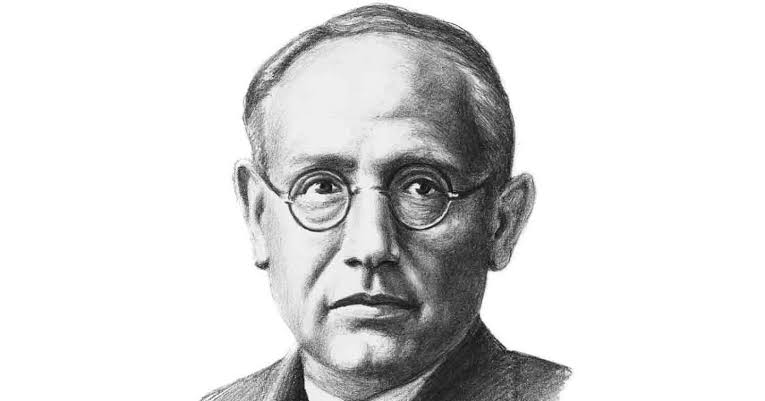
\includegraphics[width=\textwidth]{fig/ch3/gpolya.jpeg}
    \caption{G. Polya}
    \label{fig:induction}
\end{figure}
\end{column}

\end{columns}
    
\end{frame}

\begin{frame}{Jospher's Problem Generlized(JPG)}

Idea: Whenever a person is passed over, give it a \underline{new
number}. 

Demonstrate: \pause 
$$
\begin{array}{rrrrrrrrrr}1&2&3&4&5&6&7&8&9&10\\11&12&&13&14&&15&16&&17\\18&&&19&20&&&21&&22\\&&&23&24&&&&&25\\&&&26&&&&&&27\\&&&28&&&&&\\&&&29&&&&\\&&&30&&&&&\end{array}
$$
    
\end{frame}

\begin{frame}{JPG: Findings}
$$
\begin{array}{llllllllll}1&2&3^1&4&5&6^2&7&8&9^3&10\\11&12^4&&13&14&&15^5&16&&17\\18^6&&&19&20&&&21^7&&22\\&&&23&24^8&&&&&25\\&&&26&&&&&&27^9\\&&&28&&&&&\\&&&29&&&&\\&&&30^{10}&&&&&\end{array}
$$

\only<1-2>{
    What will the id become? 
    \begin{itemize}
        \item 1, 2 become \visible<2->{$n+1, n+2$};
        \item 3 executed; 
        \item 4, 5 become \visible<2->{$n+3, n+4$};
        \item 6 is executed;
        \item $3k+1, 3k+2$ will become \visible<2->{$n+2k+1, n+2k+2$};
        \item $3k+3$ is executed. 
    \end{itemize}
}

\only<3>{
\begin{itemize}
    \item Counting is consistent, no jumping over someone. 
    \item The $k$-th person eliminated ends up with number $3k$.
    \item To find the survivor = figure out the original number $3N$.
\end{itemize}
}

\only<4>{
    \begin{itemize}
        \item What is $3N$ originally? 
        \item $N(N>n)$ has a form of $N = n+2k+1$ or $N=n+2k +2$, in a single round. 
        \item for two $k$s, getting $k_1 = (N-1-n)/2, k_2=(N-2-n)/2$. 
        \item $=\flr{(N-n-1)/2}$. 
    \end{itemize}
}

\only<5>{
    An algorithm for this: 
    \begin{itemize}
        \item Let $N \leftarrow 3n$;
        \item while $N>n$, let $N\leftarrow \flr{(N-n-1)/2}+N-n$;
        \item Answer$\leftarrow N$.
    \end{itemize}
}

\only<6> {
    Simplifying this algorithm: like treating arithmetic series.
    \begin{itemize}
        \item Assign the numbers from largest to smallest
        \item yielding $\cil{3/2D}$. 
    \end{itemize}
}

\only<7> {
    Generalized: $D=\cil{q/(q-1)D}$ for general $q$s, i.e. $q$-kill one. 
}
    
\end{frame}


\section{Mod: The binary Op}

\begin{frame}{Mod: definition}
    We may rewrite the quotient and remainder as follows: 

    If $n$ is an integer, then $$n=m\flr{n/m}+n\bmod m.$$ for $y\neq 0$. 

\only<1>{
    \begin{itemize}
        \item generalize it to negative integers
        \item $5 \bmod 3 = 5-3\flr{5/3} =2.$ 
        \item $5 \bmod -3 = 5-(-3)\flr{5/-3} =-1.$ 
        \item $-5 \bmod 3 = -5-(-3)\flr{-5/3} =1.$ 
        \item $-5 \bmod -3 = -5-(-3)\flr{-5/-3} =-2.$ 
    \end{itemize}
}

\only<2>{
    \begin{itemize}
        \item Observation: In any case the result number 
        is exactly in between 2 numbers. 
        \item Special definition: if $y=0$, then $x\bmod 0=x$. 
        \item preserves the property that $x$ and $y$ 
        always differs from $x$ by a multiple of $y$.
    \end{itemize}
}
    
\end{frame}

\begin{frame}{Another notation: Mumble}
    We have $n \bmod m = n - \flr{n/m}m$

    Alternative definition: \underline{mumble}. 
    $$
    x \operatorname{ mumble } y = y \cil{{x\over y}} -x
    $$
\end{frame}

\begin{frame}{Properties}
    \begin{itemize}
        \item Distributive: $c(x\bmod y) = (cx) \bmod (cy)$
        for $c,x,y\in \R$. 
        \item reason: $c(x\bmod y) = c(x-y\cil{x/y})=cx-cy(\flr{cx/cy}) = (cx) \bmod (cy)$. 
    \end{itemize}
\end{frame}

\begin{frame}{Example: Even partition problem(EPP)}

Problem: Partition $n$ things into $m$ groups as equally
as possible. 

\only<1>{
    An example: 
    $$
    \begin{matrix}
      1&  9&   17&  25& 33\\
      2&  10&  18&  26& 34\\
      3&  11&  19&  27& 35\\
      4&  12&  20&  28& 36\\
      5&  13&  21&  29& 37\\
      6&  14&  22&  30& \\
      7&  15&  23&  31& \\
      8&  16&  24&  32&
    \end{matrix}
    $$
   \begin{itemize}
       \item  the final row has only 5 elems, can we do better? 
   \end{itemize}
}

\only<2>{
    A evener example: 
    An example: 
    $$
    \begin{matrix}
      1&  9&   17&  24& 31\\
      2&  10&  18&  25& 32\\
      3&  11&  19&  26& 33\\
      4&  12&  20&  27& 34\\
      5&  13&  21&  28& 35\\
      6&  14&  22&  29& 36\\
      7&  15&  23&  30& 37\\
      8&  16&  &      &
    \end{matrix}
    $$
}

\only<3>{
    \begin{itemize}
        \item Division: a row by row arrange not always good. 
        \item it tells us how many lines to put 
        \begin{itemize}
            \item Some of the short one put $\cil{n/m}$ columns, others put $\flr{n/m}$ cols. 
            \item There will be exactly $n \bmod m$ cols, and exactly $m-n\bmod m = n \operatorname{ mumble }m$short ones. 
        \end{itemize}
        
    \end{itemize}
}

\only<4> {
    Procedure: 
    \begin{itemize}
        \item To distribute $n$ things into 
        $m$ groups as even as possible, 
        \item when $m>0$, put $\cil{n/m}$ things into one group
        \item then use this procedure to recursively 
        \item i.e. put put the remaining $n'=n-\cil{n-m}$ things into $m'=m-1$ groups.
    \end{itemize}
    Proof: 
    \begin{itemize}
        \item Suppose that $n=qm+r$
        \item If $r=0$, We put $\flr{n/m}=q$ things into the first, $n'= n-q, m'=m-1$. 
        \item If $r>0$, put $\flr{n/m}=q+1$ into first group, leaving $n'=n-q-1=qm'+r-1$.
    \end{itemize}
}

\only<5>{
    A closed form for the formula? 
    \begin{itemize}
        \item Effect: the quotient stays the same, but the remainder decrease by 1. 
        \item That is there are $\cil{n/m}$ things when $k\leq n \bmod m$, and $\flr{n/m}$ things o.w.
        \item So the closed form is $\cil{n-k+1/m}$. 
    \end{itemize}

    Since we are arrange $n$ elems, we have the following identity: 

    $$
    n=\flr{{n\over m}}+\flr{{n+1\over m}}+\cdots+\flr{{n+(m-1)\over m}}
    $$
    
    Replace $n$ by $mx$ we get 
    
    $$
    mx=\flr{{x}}+\flr{{x+{1\over m}}}+\cdots+\flr{{x+{m-1\over m}}}
    $$
}
\end{frame}

\begin{frame}{Example: A Weird Sum(WS)}
    Find 
    $$
    \sum_{0\leq k \leq n} \flr{\sqrt{k}}
    $$where $a$ is a perfect square. 
    
    Solution:
\only<1>{
    \begin{align*}
        &~\sum_{0\leq k\leq n} \cil{\sqrt{k}} \\  
        &=\sum_{k, m\geq 0} m[k<n][m=\cil{k}] \\
        &=\sum_{k, m\geq 0} m [k<n] [m\leq \sqrt{k}<m+1]     
    \end{align*}

    Then we calculate the total number of this.
}

\only<2>{
    \begin{align*}
        &=\sum_{k, m\geq 0} m [k<n] [m\leq \sqrt{k}<m+1]  \\
        &=\sum_{k, m\geq 0} m[m\leq k \leq (m+1)^2 \leq a^2] \\
        &= \sum_{m\geq 0} m((m+1)^2-m^2)[m+1\leq a] \\ 
        &= \sum_{m\geq 0, m\leq a} m(2m+1) \\ 
    \end{align*}

    Oh, we can use falling sums! 
}

\only<3>{
    That is 
    $$
    \sum_0^a (2m^{\underline2}+3m^{\underline1})\delta m
    $$
    Using the integration rule, we get $2/3a(a-1)(a-2)+3/2a(a-1)$. 
}

\only<4> {
    Removing the perfect square condition
    \begin{itemize}
        \item do the partition from $[0..a^2]$ and $[a^2..n]$. 
        \item this will use O notation to express its increament. 
    \end{itemize}
}
    
    
\end{frame}

\begin{frame}{Example: an Integrated Example(IE)}

Find the closed form for 
$$
\sum_{0\leq k< m} \flr{{nk+x\over m}} 
$$
for integer $m>0$, integer $n$. 

\only<1>{
    We first look at some observations
    \begin{itemize}
        \item $n=1$, yields $\sum_{0\leq k<m}\flr{(k+x)/m}$, where we found at the EPP problem. 
        \item $m=1$, this will be $\flr{x}$;
        \item $m=2$, we look at $\flr{x/2}+\flr{(x+n)/2}$. 
        \begin{itemize}
            \item $n$ even, $n/2$ integer. $\flr{x/2}+\flr{(x+n)/2}=2\flr{x/2}+{n/2}$. 
            \item $n$ odd, $(n-1)/2$ integer. $\flr{x/2}+(\flr{(x+1)/2}+(n-1)/2)=\flr{x}+{(n-1)/2}$.
        \end{itemize}
    \end{itemize}
}

\only<2>{
    Have a look at $m=3$: 
    \begin{itemize}
        \item $n \bmod 3 = 0, n/3 $ and $2n/3$ integers: $\flr{{x\over3}}+\flr{{x\over3}+{n\over 3}}+\flr{{x\over3}+{2n\over 3}}=3\flr{x/3}+n$.
        \item $n \bmod 3 = 1, n-1/3 $ and $2n-2/3$ integers: $\flr{{x\over3}}+\flr{{x+1\over3}+{n-1\over 3}}+\flr{{x+2\over3}+{2n-2\over 3}}=\flr{x}+n-1$.
        \item $n \bmod 3 = 2, n-2/3 $ and $2n-4/3$ integers: $\flr{{x\over3}}+\flr{{x+2\over3}+{n-2\over 3}}+\flr{{x+4\over3}+{2n-4\over 3}}=\flr{x}+n-1$.
    \end{itemize}
}

\only<3>{
    Look at $n=4$, 
    \begin{itemize}
        \item $n\bmod 4 = 0, 4\flr{x/4}+3n/2$;
        \item $n\bmod 4 = 1, \flr{x}+3n/2-3/2$;
        \item $n\bmod 4 = 0, \flr{x}+3n/2-3/2$;
        \item $n\bmod 4 = 0, 2\flr{x}+3n/2-1$;
    \end{itemize}
}

\only<4>{
    We make a small table for this: 
    $$
    \begin{array}{c|cccc}m &n \bmod m = 0&n \bmod m = 1&n \bmod m=2&n \bmod m==3\\
    \hline 
    1 &\lfloor x \rfloor\\
    2&2\left\lfloor\frac x2\right\rfloor+\frac n2&\lfloor x \rfloor+\frac n2-\frac12\\
    3&3\left\lfloor\frac x3\right\rfloor+n &\lfloor x \rfloor+n -1&\lfloor x \rfloor+n -1\\4&4\left\lfloor\frac x4\right\rfloor+\frac{3n }2&\lfloor x \rfloor+\frac{3n }2-\frac32&2\left\lfloor\frac x2\right\rfloor+\frac{3n }2-1&\lfloor x \rfloor+\frac{3n }2-\frac32\end{array}
    $$
    It looks that: 
    $$
    \flr{\frac{x+kn\bmod m}{m}+\frac{kn}{m}-\frac{kn\bmod m}{m}}
    $$
}

\only<5>{
    This can be extracted from
    $$
    \flr{\frac{x+kn\bmod m}{m}}+\frac{kn}{m}-\frac{kn\bmod m}{m}
    $$
}

\only<6> {
    $$
    \small
    \begin{aligned}
    & \left\lfloor\frac{x}{m}\right\rfloor&+\frac{0}{m}&-\frac{0 \bmod m}{m} \\
    + & \left\lfloor\frac{x+n \bmod m}{m}\right\rfloor&+\frac{n}{m}&-\frac{n \bmod m}{m} \\
    + & \left\lfloor\frac{x+2 n \bmod m}{m}\right\rfloor&+\frac{2 n}{m}&-\frac{2 n \bmod m}{m} \\
    &\vdots & \vdots \\
    + & \underbrace{\left\lfloor\frac{x+(m-1) n \bmod m}{m}\right\rfloor}_{a\left\lfloor\frac{x}{a}\right\rfloor}&+\underbrace{\frac{(m-1) n}{m}}_{b n}&-\underbrace{\frac{(m-1) n \bmod m}{m}}_C .
    \end{aligned}
    $$

}

\only<7>{
    Looking at the table: 
    \begin{itemize}
        \item The second column is $\frac{1}{2}\left(0+\frac{(m-1) n}{m}\right) m$
        \item The first column: See what $0 \bmod m, \quad n \bmod m, 2 n \bmod m, \cdots,(m-1) n \bmod m$ will get. 
    \end{itemize}
    
}

\only<8>{
    Look at the first row of that one, recall 
    $$
    \small
    n=\left\lfloor\frac{n}{m}\right\rfloor+\left\lfloor\frac{n+1}{m}\right\rfloor+\cdots+\left\lfloor\frac{n+(m-1)}{m}\right\rfloor
    $$

    \begin{itemize}
        \item We will encounter the remainder from $1$ to $n$ one time(we will show at Chapt. 4)
    \end{itemize}
}

\only<9> {
    So we have: 
    $$
    \small
    \begin{aligned}
    & d\left(\left\lfloor\frac{x}{m}\right\rfloor+\left\lfloor\frac{x+d}{m}\right\rfloor+\cdots+\left\lfloor\frac{x+m-d}{m}\right\rfloor\right) \\
    = & d\left(\left\lfloor\frac{x / d}{m / d}\right\rfloor+\left\lfloor\frac{x / d+1}{m / d}\right\rfloor+\cdots+\left\lfloor\frac{x / d+m / d-1}{m / d}\right\rfloor\right) \\
    = & d\left\lfloor\frac{x}{d}\right\rfloor ., \text { and hence, } a=d=\operatorname{gcd}(m, n) .
    \end{aligned}
    $$
}

\only<10>{
    The third column: $d\left(\frac{1}{2}\left(0+\frac{m-d}{m}\right) \cdot \frac{m}{d}\right)=\frac{m-d}{2}$

    \begin{itemize}
        \item $c=\frac{d-m}{2}$.
    \end{itemize}

    
}

\only<11> {
    Putting altogether: 
    $$\sum_{0 \leqslant k<m}\left\lfloor\frac{n k+x}{m}\right\rfloor=d\left\lfloor\frac{x}{d}\right\rfloor+\frac{m-1}{2} n+\frac{d-m}{2}.$$

    where $d=\operatorname{gcd}(m, n)$.

    
}

\only<12> {
    In fact, $m$ and $n$ are symmetric: 
    $$
    \small
\begin{aligned}
\sum_{0 \leqslant k<m}\left\lfloor\frac{n k+x}{m}\right\rfloor & =d\left\lfloor\frac{x}{d}\right\rfloor+\frac{m-1}{2} n+\frac{d-m}{2} \\
& =d\left\lfloor\frac{x}{d}\right\rfloor+\frac{(m-1)(n-1)}{2}+\frac{m-1}{2}+\frac{d-m}{2} \\
& =d\left\lfloor\frac{x}{d}\right\rfloor+\frac{(m-1)(n-1)}{2}+\frac{d-1}{2}
\end{aligned}
$$

saying, 

$$
\small
\sum_{0 \leqslant k<m}\left\lfloor\frac{n k+x}{m}\right\rfloor=\sum_{0 \leqslant k<n}\left\lfloor\frac{m k+x}{n}\right\rfloor, \quad \text { integers } m, n>0 \text {. }
$$
}

\end{frame}



\begin{frame}[plain]
    $$
    \Huge \textbf{Thanks}
    $$
  \end{frame}

\end{document}
